\documentclass[main]{subfiles}

\begin{document}


\chapter{Linealizaci\'on y puntos de operaci\'on}
\label{chap:linealizacion}

Independientemente del sistema bajo estudio, a la hora de elegir la t\'ecnica de control a utilizar se plantean diversas posibilidades. Parece razonable intentar resolver el problema planteado utilizando las t\'ecnicas m\'as sencillas de las que se disponen, al menos en una primera aproximaci\'on. En caso de que dicha soluci\'on no fuese satisfactoria se puede optar por una t\'ecnica con un mayor grado de complejidad.\\ 

Las t\'ecnicas de control m\'as sencillas y con las que se tiene mayor experiencia se basan en el estudio de sistemas lineales invariantes en el tiempo (SLIT). El MVE obtenido en el cap\'itulo \ref{chap:modelo} es no lineal, por lo que se propone resolver el problema del control del cuadric\'optero aproximando el sistema por un sistema lineal invariante en el tiempo. En una primera instancia se centrar\'a el an\'alisis en determinar bajo qu\'e condiciones es posible aproximar el sistema por un SLIT.

\section{Concepto general}
Dado un sistema que se rige por la siguiente evoluci\'on de su vector de estados:
\begin{equation}
\dot{x}(t)=f(x(t),u(t))
\end{equation}

Donde $x(t)$ es el vector de estados del sistema y $u(t)$ el vector de las entradas. Suponiendo, en una primera instancia, que tanto $x(t)$ como $u(t)$ son de dimensi\'on uno y considerando adem\'as el punto de operaci\'on definido por $x^*(t)$ y $u^*(t)$, un desarrollo de Taylor de \'orden uno en torno al punto de operaci\'on resulta en:
\begin{equation}
\dot{x}(t)=f(x(t),u(t))=f(x^*(t),u^*(t))+\frac{\partial f}{\partial x}\vert_{u=u^*}^{x=x^*}(x(t)-x^*(t))+\frac{\partial f}{\partial u}\vert_{u=u^*}^{x=x^*}(u(t)-u^*)
\end{equation}

Definiendo $\tilde{x}(t)=x(t)-x^*(t)$ y $\tilde{u}(t)=u(t)-u^*(t)$ se obtiene que:

\begin{equation}
\dot{\tilde{x}}(t)=\frac{\partial f}{\partial x}\vert_{u=u^*}^{x=x^*}\tilde{x}(t)+\frac{\partial f}{\partial u}\vert_{u=u^*}^{x=x^*}\tilde{u}(t)
\end{equation}

Este mismo concepto puede generalizarse al caso en el cual el vector de estados y el vector de entradas tienen dimension n y m respectivamente.
\begin{equation}
\dot{\tilde{X}}(t)=A(t)\tilde{X}(t)+B(t)\tilde{U}(t)
\end{equation}
Donde $A(t)$ es una matriz de $n \times n$ y $B(t)$ es de $n \times m$, tales que $a_{ij}= \frac{\partial f_i}{\partial X_j}\vert_{U=U^*}^{X=X^*}$ y  $b_{ij}= \frac{\partial f_i}{\partial U_j}\vert_{U=U^*}^{X=X^*}$.\\

En el caso en que todos los coeficientes de las matrices A y B son constantes es posible afirmar que el sistema es lineal e invariante en el tiempo. 

\section{Puntos de operaci\'on}
Se buscan trayectorias tales que la linealizaci\'on del sistema en torno a ellas resulte en un sistema lineal invariante en el tiempo.\\

Para lograr este cometido, se debe cumplir que todos los elementos de las matrices \ref{eq:Agenerica} y \ref{eq:Bgenerica} del anexo \ref{chap:anexo_linealizacion} sean constantes. Dichas matrices corresponden a la linealizaci\'on del MVE en torno a una trayectoria gen\'erica. Se desprende del an\'alisis de dichas matrices que los puntos de operaci\'on que cumplen esta condici\'on quedan restrictos a un subconjunto tal que:
\begin{equation}
\dot{\psi}=\dot{\varphi}=\dot{\theta}=\dot{v}_{qx}=\dot{v}_{qy}=\dot{v}_{qz}=\dot{\omega}_{qx}=\dot{\omega}_{qy}=\dot{\omega}_{qz}=\dot{\omega}_1=\dot{\omega}_2=\dot{\omega}_3=\dot{\omega}_4=0
\end{equation}
Luego se ver\'a que, realizando un cambio de variable como se explica en \cite{bib:auion}, se puede ampliar el conjunto de trayectorias posibles, pudiendo agregar aquellas para las cuales $\dot{\theta} \neq 0$. Estas consideraciones llevan a concluir que el conjunto de trayectorias permitidas\footnote{por la restricci\'on de trabajar con un sistema lineal invariante en el tiempo.} es aquel en el cual tanto la velocidad del centro de masa, como la velocidad angular son constantes en el tiempo. Las trayectorias que cumplen con estas condiciones son tres:

\begin{itemize}
\item Hovering
\item Vuelo en linea recta a velocidad constante
\item Vuelo en c\'irculo a velocidad constante 
\end{itemize} 

En los tres casos se tienen que cumplir las restricciones siguientes:
\begin{equation}
\label{eq:slit}
\left(\begin{array}{c}
\dot{v}_{qx}\\
\dot{v}_{qy}\\
\dot{v}_{qz}\\
\end{array}\right)=0 \quad 
\left(\begin{array}{c}
\dot{\omega}_{qx}\\
\dot{\omega}_{qy}\\
\dot{\omega}_{qz}\\
\end{array}\right)=0
\end{equation}
Cada una de las trayectorias posibles tiene adem\'as sus particularidades, a continuaci\'on se determinan las restricciones espec\'ificas de cada una de ellas.

\subsection{Hovering}
En el caso del reposo mec\'anico no solo deben cumplirse las condiciones establecidas en \ref{eq:slit} sino que adem\'as las velocidades del centro de masa y las velocidades angulares deben ser iguales a cero:
\begin{equation}
\label{eq:quieto}
\left(\begin{array}{c}
v_{qx}\\
v_{qy}\\
v_{qz}\\
\end{array}\right)=0 \quad
\left(\begin{array}{c}
\omega_{qx}\\
\omega_{qy}\\
\omega_{qz}\\
\end{array}\right)=0
\end{equation}

Dado que la velocidad y velocidad angular del sistema fueron definidas como cero, s\'olo quedan por determinar 7 variables: los \'angulos de Euler y las velocidades angulares de los motores. \\

Al imponer las condiciones de \ref{eq:quieto}, las ecuaciones \ref{eq:euler} y \ref{eq:pospunto} del MVE se cumplen trivialmente. La restricci\'on establecida en \ref{eq:slit} consta de seis ecuaciones. Estas no dependen de $\theta$, obteniendo entonces un sistema de seis ecuaciones y seis inc\'ognitas que debe ser resuelto a fin de determinar las condiciones que permiten el hovering. Ninguna de las seis ecuaciones depende de la posici\'on  lo cual, sumado a la independencia de la condici\'on de hovering respecto de $\theta$, permite confirmar un resultado evidente: \textbf{el hovering puede lograrse en cualquier punto del espacio con cualquier \'angulo de Yaw}\\

Del an\'alisis de las ecuaciones \ref{eq:slit} se obtiene que:
\begin{equation}
\varphi=0 \quad \psi=0 \quad \omega_1=\omega_2=\omega_3=\omega_4=\omega_{hover}
\end{equation}


\subsection{Vuelo en linea recta a velocidad constante}

Cabe recordar que el modelo desarrollado no incluye ninguna fuerza aerodin\'amica a excepci\'on de aquellas que producen las fuerzas y los torques sobre las h\'elices. Bajo esta suposici\'on las condiciones necesarias para lograr rectas y c\'irculos difieren sensiblemente de la realidad. Para lograr el vuelo en linea recta a velocidad constante se tienen que cumplir las condiciones de \ref{eq:slit}, al igual que en el caso anterior. La particularidad del vuelo en linea recta es que la velocidad del centro de masa es una constante distinta de cero. 
\begin{equation}
\label{eq:recta}
\left(\begin{array}{c}
v_{qx}\\
v_{qy}\\
v_{qz}\\
\end{array}\right)=cte \quad
\left(\begin{array}{c}
\omega_{qx}\\
\omega_{qy}\\
\omega_{qz}\\
\end{array}\right)=0
\end{equation}
Al imponer que $\vec{\omega}_q=0$ la ecuaci\'on \ref{eq:euler} se verifica trivialmente y las ecuaciones \ref{eq:vpuntos} y \ref{eq:omegas} quedan id\'enticas al caso del sistema en reposo. Por lo tanto, al igual que para el hovering, se tendr\'a que:
\begin{equation}
\varphi=0 \quad ; \quad \psi=0 \quad ; \quad \omega_1=\omega_2=\omega_3=\omega_4 = \omega_{hover}
\end{equation}

Hasta aqu\'i no se ha considerado la ecuaci\'on que relaciona las velocidades lineales en el sistema inercial con las velocidades lineales expresadas en el sistema del cuadric\'optero. Teniendo presente el resultado obtenido sobre $\varphi$ y $\psi$ dichas ecuaciones toman la forma:
\begin{equation}\begin{array}{c}
\dot{x}=v_{q_x}\cos\theta-v_{q_y}\sin\theta\\
\dot{y}=v_{q_y}\sin\theta+v_{q_y}\cos\theta\\
\dot{z}=v_{q_z}
\end{array}
\end{equation} 

Se deduce entonces que el vuelo en l\'inea recta queda determinado al fijar las restantes 4 variables del sistema: $v_{q_x}$, $v_{q_y}$, $v_{q_z}$ y $\theta$. Estos par\'ametros ser\'an determinados por el generador de trayectorias con el objetivo de realizar una recta en particular con una orientaci\'on determinada. 

\subsection{Vuelo en c\'irculos}

Con las ecuaciones desarrolladas hasta ahora no resulta posible realizar movimientos con velocidades angulares distintas de cero sin que el sistema resultante sea variante en el tiempo. Si se impone que la velocidad angular del sistema sea distinta a cero se tiene que al menos una de las derivadas de los \'angulos de Euler es distinta de cero y por lo tanto se tendr\'a al menos un \'angulo de Euler variante en el tiempo. Para poder obtener un movimiento circular se realiza el cambio de variable en el MVE en lo que respecta a las ecuaciones de la derivada de la posici\'on propuesto en \cite{bib:auion}. \\

\begin{wrapfigure}{l}{0.50\textwidth}
  \begin{center}
  \vspace{-10pt}
    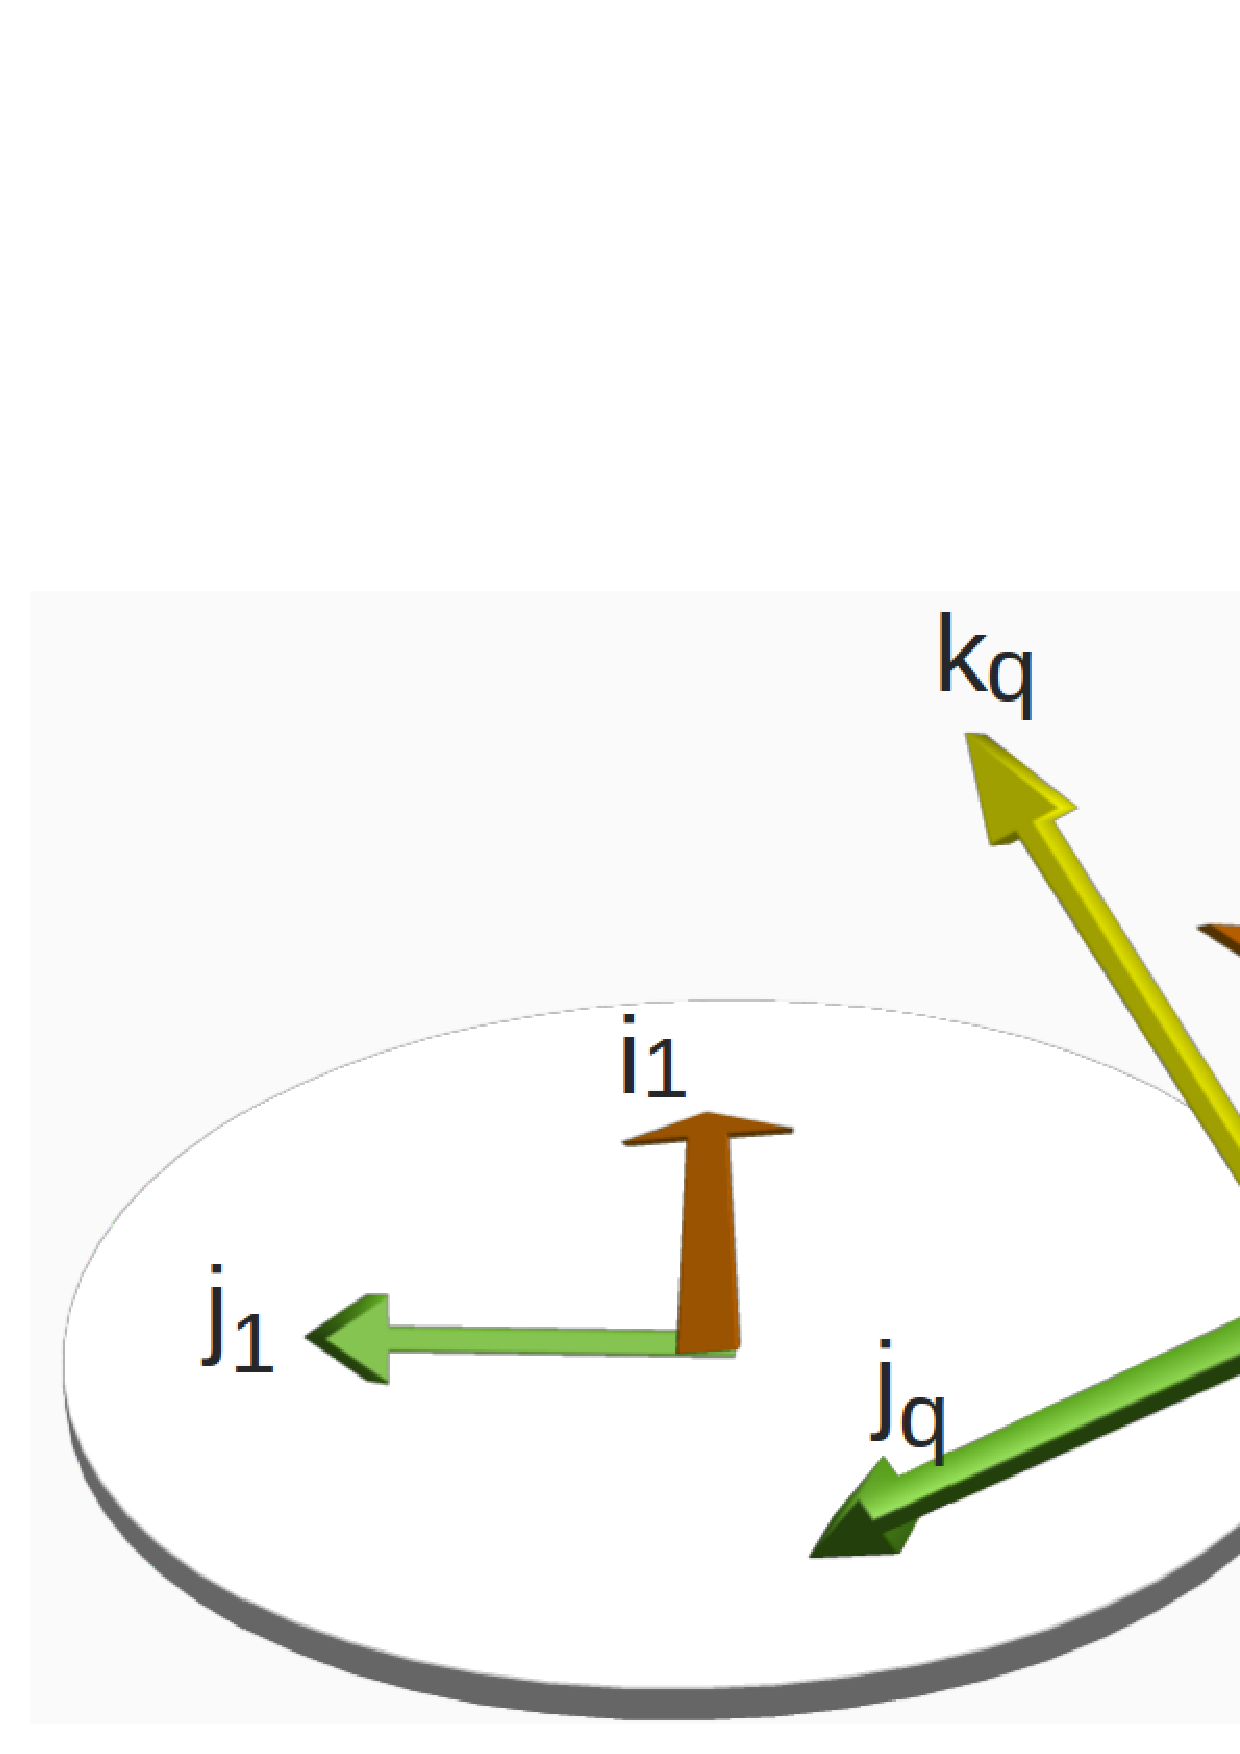
\includegraphics[width=0.40\textwidth]{./pics_linealizacion/circulo.pdf}
  \end{center}
  \caption{Vuelo en c\'iculo}
  \label{fig:circulo}
\end{wrapfigure}

El cambio de variable en cuesti\'on consiste en expresar la posici\'on (exclusivamente para los movimientos circulares) en la base del cuadric\'optero. Suponiendo que el cuadric\'optero se encuentra realizando un movimiento tal que su proyecci\'on sobre el plano horizontal ($z=0$) es circular, se puede describir la posici\'on en todo momento tomando como origen el centro de dicho c\'irculo. Como se observa en la figura \ref{fig:circulo} la posici\'on en dicho plano se puede expresar como $-R\vec{j}_1$\footnote{Esto es debido a que se elige que el vector $\vec{i}_q$ sea tangente a los c\'irculos descriptos. El razonamiento es an\'alogo si se desea que el vector $\vec{j}_q$ sea tangente al c\'irculo, en este caso debe expresarse la posic\'on del sistema como $R\vec{i}_1$}. Donde $R$, es el radio del c\'irculo y $\vec{j}_1$ es un vector de la base que se obtiene al realizar la primera rotaci\'on de Euler definida en \ref{eq:bases}. Multiplicando el vector $-R\vec{j_1}$ por la matriz cambio de base $H_2^qH_1^2$ definida en \ref{eq:bases} se obtiene la posici\'on expresada en el sistema $S_q$. Como $\vec{j}_1$ es invariante frente a la rotaci\'on $H_1^2$, alcanza con multiplicar dicho vector por $H_2^q$ obteniendo as\'i:
\begin{equation}
\label{eq:pos_circ}
\vec{r}_q=-H_2^q\vec{i}_1=-R\left(\begin{array}{c}
0\\
\cos\psi\\
-\sin\psi\\
\end{array}\right)
\end{equation}
Al expresar la posici\'on con este cambio de variables se obtiene la independencia de la misma respecto de dos de los tres \'anglos de Euler: $\varphi$ y $\theta$. En lo que respecta al \'angulo $\varphi$ la independencia de esta variable no aporta absolutamente nada ya que para que el movimiento circular a velocidad constante sea posible dicho \'angulo debe ser cero. La raz\'on es que si el \'angulo fuese diferente a cero se tendr\'ia una componente de la fuerza en la direcci\'on tangencial al c\'irculo, y por lo tanto una aceleraci\'on en dicha direcci\'on.\\

La independencia respecto de $\theta$ en la posici\'on es un paso fundamental para lograr el vuelo en c\'irculos ya que las \'unicas ecuaciones del MVE (\ref{eq:modelo}) que dependen de esta variable son las que refieren a la derivada de la posici\'on. Por lo tanto, ser\'a posible desarrollar un nuevo MVE independiente del \'angulo de Yaw.\\

Interesa ahora derivar la posici\'on para terminar de completar el modelo del sistema. Dado que la posici\'on se encuentra expresada en el sistema del cuadric\'optero, se tiene que:
\begin{equation}
\vec{v}_q = \frac{d\vec{r}_q}{dt}=\frac{d^\prime\vec{r}_q}{dt}+\vec{\omega}_q \times \vec{r}_q
\end{equation}
y por lo tanto:
\begin{equation}
\label{eq:MVEcirc}
\left(\begin{array}{c}
\dot{x_q}\\
\dot{y_q}\\
\dot{z_q}\\
\end{array}\right)=\left(\begin{array}{c}
v_{q_x}-\omega_{q_y}z_q+\omega_{q_z}y_q\\
v_{q_y}-\omega_{q_z}x_q+\omega_{q_x}z_q\\
v_{q_z}-\omega_{q_x}y_q+\omega_{q_y}x_q\\
\end{array}\right)
\end{equation}

Este modelo permite realizar el control basado en t\'ecnicas de control lineal para trayectorias circulares en planos tales que $z=cte$.\\

Es fundamental aclarar que las ecuaciones derivadas hasta aqu\'i ser\'an utilizadas exclusivamente para la linealizaci\'on del sistema y no para el control. Para esto \'ultimo se continuar\'a utilizando el modelo de \ref{eq:modelo}. El movimiento circular queda determinado exclusivamente por dos par\'ametros: la velocidad ($V_I$) y la velocidad angular ($\dot{\theta}$), estos ser\'an considerados conocidos ya que es trabajo del generador de rutas o del usuario determinar que movimiento se desea realizar. Se desea determinar once par\'ametros: siete de las doce variables de estado (No interesa fijar ni \'angulo de Yaw ni la posici\'on y ya fue determinado que $\varphi = 0$) y las cuatro velocidades angulares de los motores.  Se deben tener en cuenta las restricciones establecidas en \ref{eq:slit} sobre las derivadas de las velocidades del centro de masa y de las velocidades angulares. En lo que respecta a las derivadas de los \'angulos de Euler se debe cumplir que $\dot{\varphi}=\dot{\psi}=0$, adem\'as $\dot{\theta}$ debe ser igual al valor impuesto. De $\dot{\psi} = 0$ se deduce trivialmente que $\omega_{q_x} = 0$ 

Para cada instante se tendr\'a un \'angulo de Yaw distinto, por lo tanto la velocidad horizontal a cada instante tendr\'a una direcci\'on distinta, y su m\'odulo ser\'a constante. Sin p\'erdida de generalidad podemos considerar la situaci\'on evaluando $\theta = 0$
\begin{equation}
\label{eq:vel_theta}
\left(\begin{array}{c}
v_{q_x}+v_{q_y}\sin\psi\\
v_{q_y}\cos\psi-v_{q_z}\sin\psi\\
v_{q_y}\sin\psi+v_{q_z}\cos\psi\\
\end{array}\right)=\left(\begin{array}{c}
V_{I}\\
0\\
0\\
\end{array}\right)
\end{equation}	

De la imposici\'on de dicha condici\'on surge:
\begin{equation}
v_{q_y} = - \tan^2\psi \quad v_{q_y}
\end{equation}
La soluci\'on de dicha ecuaci\'on es: $v_{q_y} = 0$, y por lo tanto $v_{q_z} = 0$ y $v_{q_x} = V_I$.\\

La soluci\'on trivial $\psi=0$ no es de inter\'es para el vuelo en c\'irculos ya que, si se impone dicha condici\'on es imposible producir una fuerza en alg\'un sentido distinto que seg\'un la vertical, no pudi\'endose realizar una fuerza centr\'ipeta necesaria para lograr un movimiento circular.\\

Resta por determinar tres de las variables de estado ($\psi, \omega_{q_y}$ y $\omega_{q_z}$) y las velocidades angulares de los motores, para lo cual se utilizar\'an las siete ecuaciones restantes del modelo f\'isico. El sistema no ser\'a resuelto en forma anal\'itica, sino en forma num\'erica a la hora de planificar la trayectoria.\\[20pt]

Hasta aqu\'i se han definido tres tipos de trayectorias, desde las cuales es posible definir y entender el comportamiento del cuadric\'optero desde el ``mundo'' del control lineal, lo que significa un paso fundamental en camino de lograr controlar el cuadric\'optero. Las trayectorias definidas ofrecen una amplia gama de posibilidades, ya que concatenando las mismas se pueden obtener pr\'acticamente cualquier movimiento, a excepci\'on de maniobras que involucren variaciones en m\'as de un \'angulo de Euler a la vez. El subconjunto de trayectorias con el que se puede trabajar es considerado ampliamente satisfactorio y por ende se da por conclu\'ido el an\'alisis sobre los puntos de operaciones y la linealizaci\'on del sistema. 

\end{document}